\section{Solución}

\subsection{Descripción}
Como se mencionó anteriormente se espera \textbf{una escalabilidad horizontal} y
principalmente una \textbf{alta disponibilidad (99.5\%)}, además de esto el
cliente requiere de desplegarlo en \textit{AWS}. \\

Por lanto, decidimos usar un \textit{balanceador de cargas clásico} de
\textit{AWS} para desplegar los \textit{EC2} (Una instancia virtual de un
servidor de Amazon) requeridos por la organización. Por lo que decidimos
desplegar la siguiente arquitectura:

\begin{figure}[H]
    \centering
    \begin{subfigure}[b]{0.8\textwidth}
        \centering
        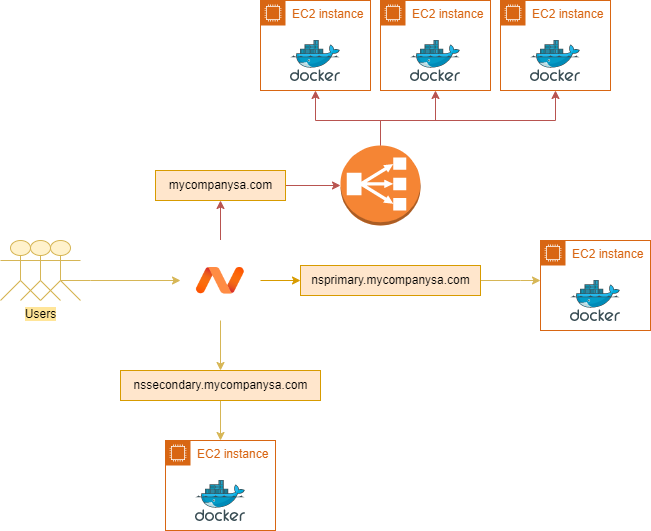
\includegraphics[width=\textwidth]{Figures/0. General/mycompanysa_architecture.png}
        \caption{\textit{Arquitectura de mycompanysa}}
        \label{fig: mycompanysa architecture}
    \end{subfigure}
\end{figure}

\subsection{Configuración}
En el siguiente apartado se documentará el proceso de cómo se hizo, esto ya sea
para una replica del proceso a futuros proyectos o para la mejora del mismo 
proyecto. \\

\subsubsection{Compra del dominio}
Lo primero que se realizó fue la compra del dominio, una de las mejores ofertas
las ofrece \textit{Namecheap}, además de que el equipo ya contaba con cierta
experiencia con esta empresa. Los pasos realizados fueron:

\begin{itemize}
    \item Registro en la plataforma.
    \item Búsqueda del dominio deseado.
    \item Compra del dominio deseado.
    \item Configuración del dominio 
\end{itemize}

Ahora bien, los 3 primeros pasos son casi mecánicos para casis cualquier compra
en línea, pero ¿cómo realizamos el último paso? Bueno, lo primero que haremos es
ingresar a nuestro dominio y nos vamos a \textit{Configuración Avanzada}.

\begin{figure}[H]
    \centering
    \begin{subfigure}[b]{0.8\textwidth}
        \centering
        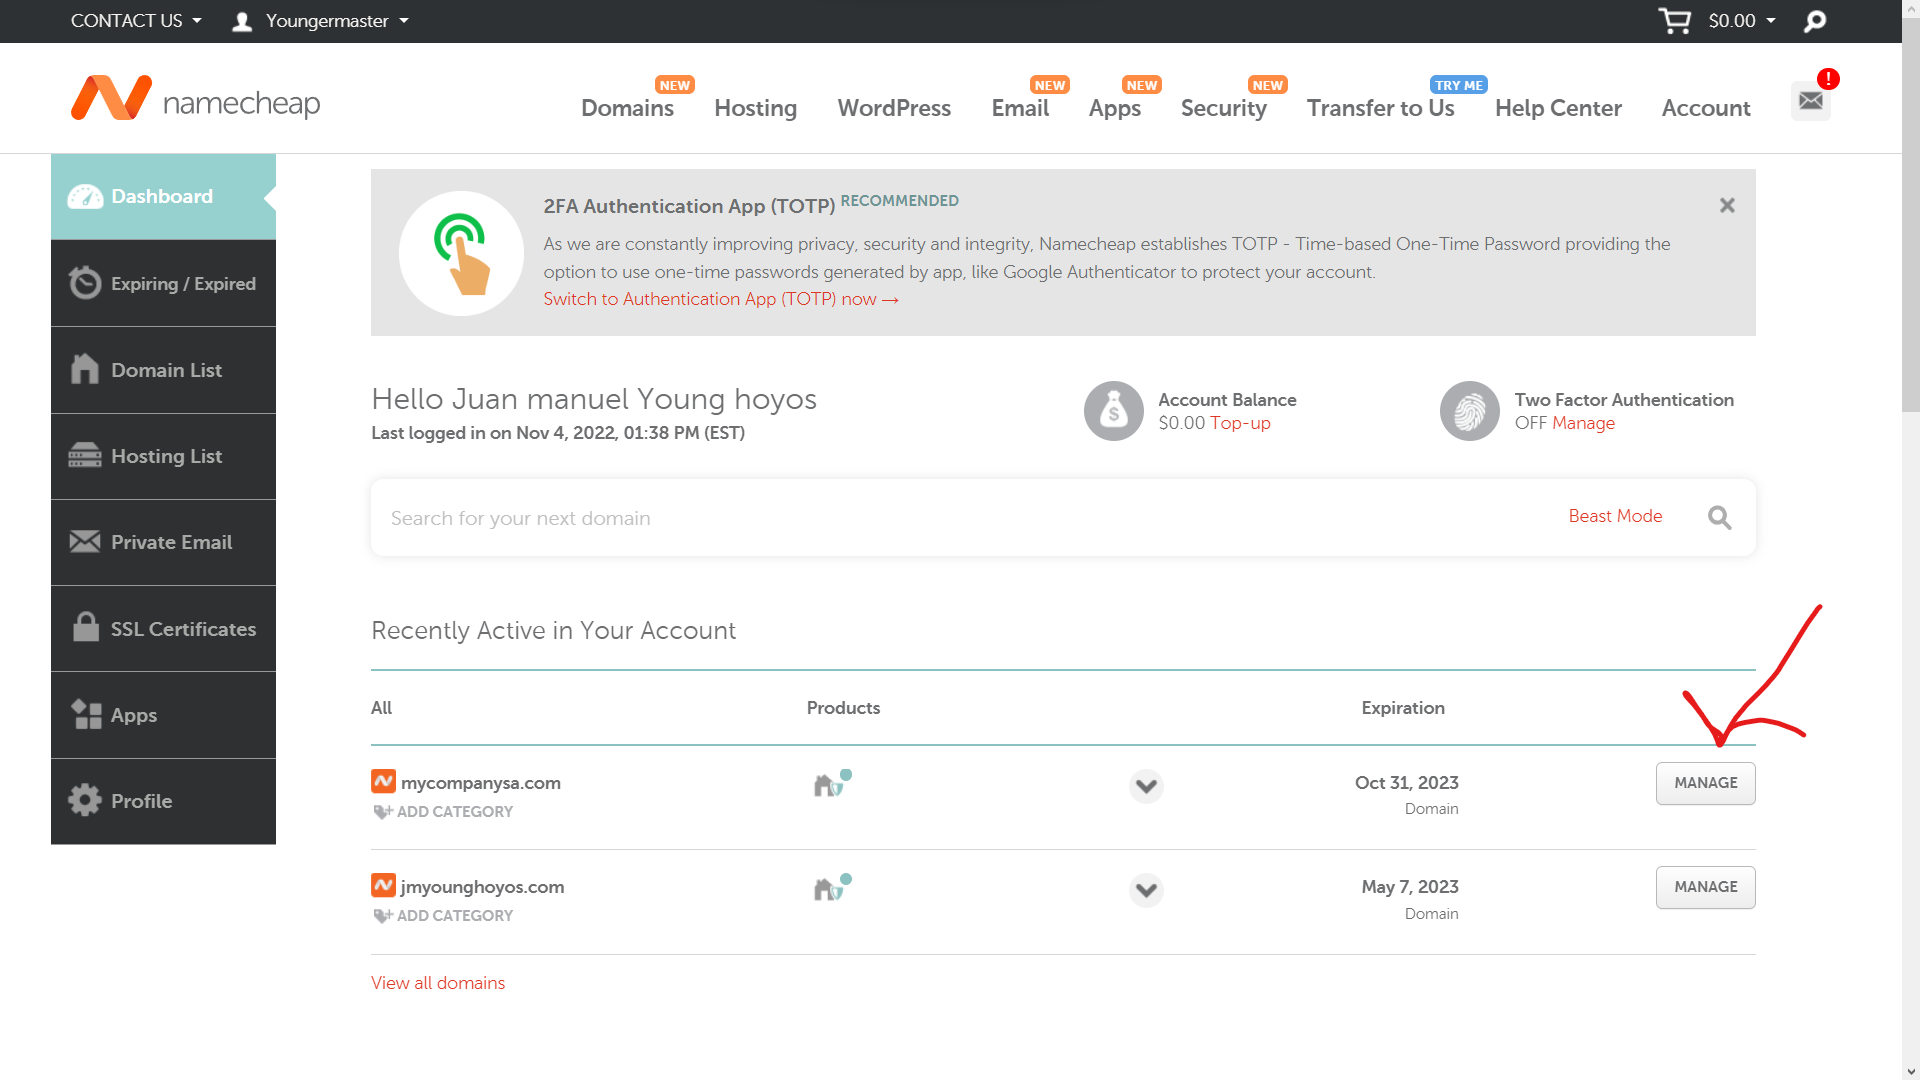
\includegraphics[width=\textwidth]{Figures/0. General/domain_selection.png}
        \caption{\textit{Selección del dominio}}
        \label{fig: domain selection}
    \end{subfigure}
\end{figure}

\begin{figure}[H]
    \centering
    \begin{subfigure}[b]{0.8\textwidth}
        \centering
        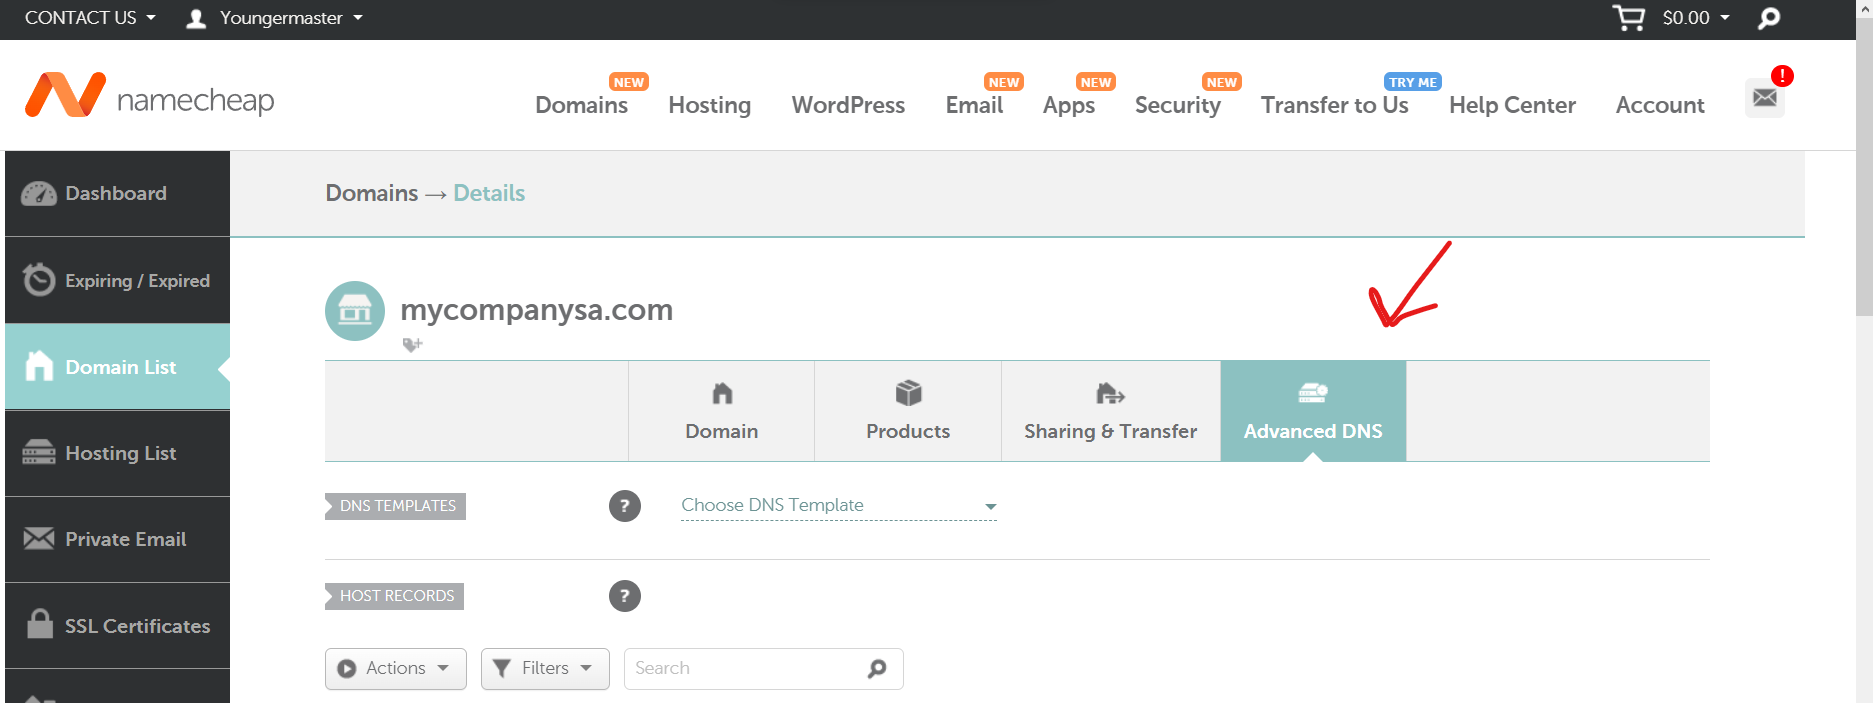
\includegraphics[width=\textwidth]{Figures/0. General/advanced_config_selection.png}
        \caption{\textit{Opción de configración avanzada de DNS}}
        \label{fig: advanced dns configuration}
    \end{subfigure}
\end{figure}

Después de esto añadiremos las siguientes rutas:

\begin{figure}[H]
    \centering
    \begin{subfigure}[b]{0.8\textwidth}
        \centering
        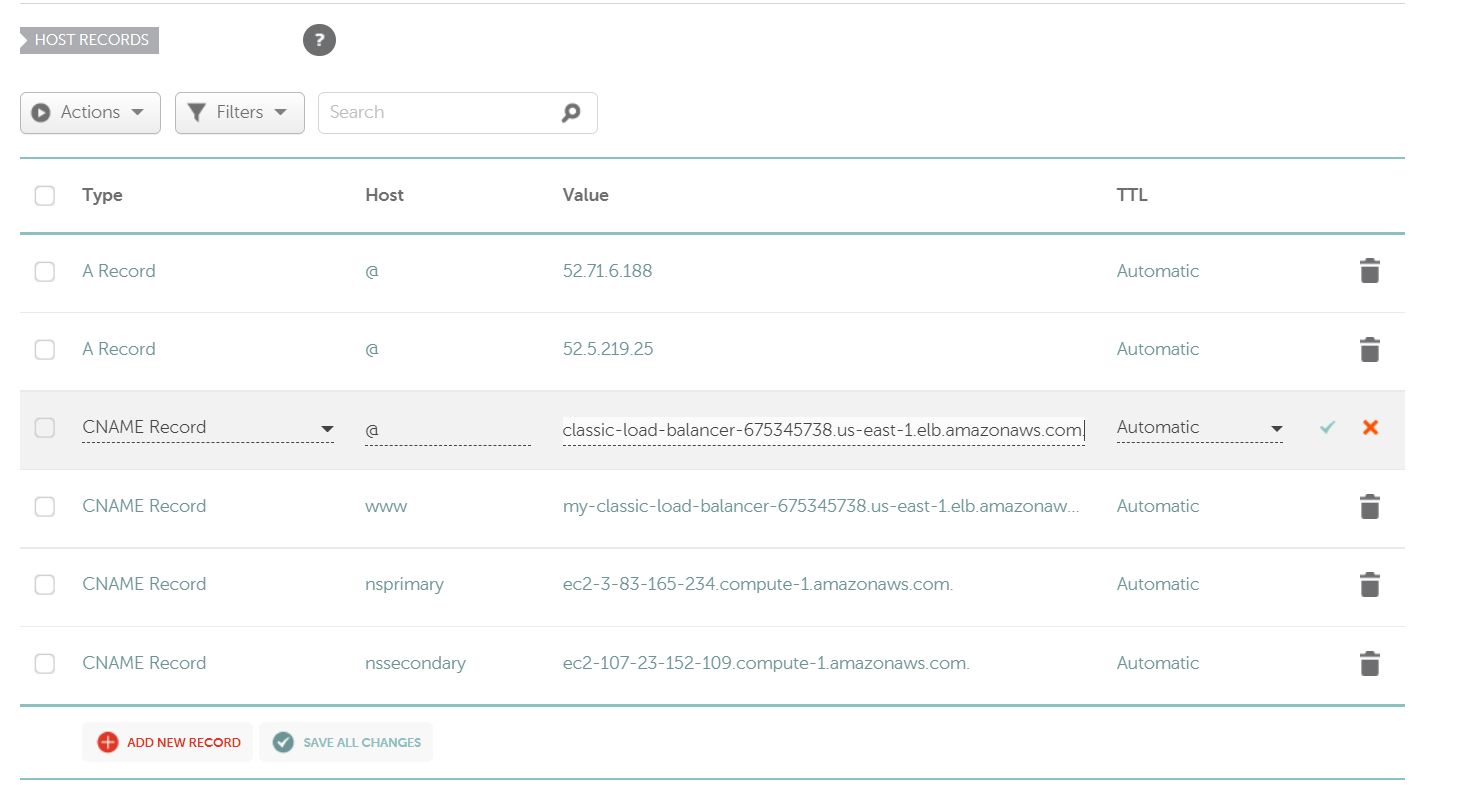
\includegraphics[width=\textwidth]{Figures/0. General/domain_config.png}
        \caption{\textit{Configración del dominio y subdominio en Namecheap}}
        \label{fig: domain configuration}
    \end{subfigure}
\end{figure}

\subsection{Demo}